% Options for packages loaded elsewhere
\PassOptionsToPackage{unicode}{hyperref}
\PassOptionsToPackage{hyphens}{url}
%
\documentclass[
]{article}
\usepackage{lmodern}
\usepackage{amssymb,amsmath}
\usepackage{ifxetex,ifluatex}
\ifnum 0\ifxetex 1\fi\ifluatex 1\fi=0 % if pdftex
  \usepackage[T1]{fontenc}
  \usepackage[utf8]{inputenc}
  \usepackage{textcomp} % provide euro and other symbols
\else % if luatex or xetex
  \usepackage{unicode-math}
  \defaultfontfeatures{Scale=MatchLowercase}
  \defaultfontfeatures[\rmfamily]{Ligatures=TeX,Scale=1}
\fi
% Use upquote if available, for straight quotes in verbatim environments
\IfFileExists{upquote.sty}{\usepackage{upquote}}{}
\IfFileExists{microtype.sty}{% use microtype if available
  \usepackage[]{microtype}
  \UseMicrotypeSet[protrusion]{basicmath} % disable protrusion for tt fonts
}{}
\makeatletter
\@ifundefined{KOMAClassName}{% if non-KOMA class
  \IfFileExists{parskip.sty}{%
    \usepackage{parskip}
  }{% else
    \setlength{\parindent}{0pt}
    \setlength{\parskip}{6pt plus 2pt minus 1pt}}
}{% if KOMA class
  \KOMAoptions{parskip=half}}
\makeatother
\usepackage{xcolor}
\IfFileExists{xurl.sty}{\usepackage{xurl}}{} % add URL line breaks if available
\IfFileExists{bookmark.sty}{\usepackage{bookmark}}{\usepackage{hyperref}}
\hypersetup{
  pdftitle={Spread of the SARS-CoV-2 Omicron (B.1.1.529) Variant in Austria},
  hidelinks,
  pdfcreator={LaTeX via pandoc}}
\urlstyle{same} % disable monospaced font for URLs
\usepackage[margin=1in]{geometry}
\usepackage{longtable,booktabs}
% Correct order of tables after \paragraph or \subparagraph
\usepackage{etoolbox}
\makeatletter
\patchcmd\longtable{\par}{\if@noskipsec\mbox{}\fi\par}{}{}
\makeatother
% Allow footnotes in longtable head/foot
\IfFileExists{footnotehyper.sty}{\usepackage{footnotehyper}}{\usepackage{footnote}}
\makesavenoteenv{longtable}
\usepackage{graphicx,grffile}
\makeatletter
\def\maxwidth{\ifdim\Gin@nat@width>\linewidth\linewidth\else\Gin@nat@width\fi}
\def\maxheight{\ifdim\Gin@nat@height>\textheight\textheight\else\Gin@nat@height\fi}
\makeatother
% Scale images if necessary, so that they will not overflow the page
% margins by default, and it is still possible to overwrite the defaults
% using explicit options in \includegraphics[width, height, ...]{}
\setkeys{Gin}{width=\maxwidth,height=\maxheight,keepaspectratio}
% Set default figure placement to htbp
\makeatletter
\def\fps@figure{htbp}
\makeatother
\setlength{\emergencystretch}{3em} % prevent overfull lines
\providecommand{\tightlist}{%
  \setlength{\itemsep}{0pt}\setlength{\parskip}{0pt}}
\setcounter{secnumdepth}{5}
\usepackage{float}
\usepackage[section]{placeins}
\usepackage{authblk}
\author{Fabian Valka \\ fvalka@vektorraum.com}
\affil{vektorraum}
\usepackage{float}
\usepackage{booktabs}
\usepackage{longtable}
\usepackage{array}
\usepackage{multirow}
\usepackage{wrapfig}
\usepackage{colortbl}
\usepackage{pdflscape}
\usepackage{tabu}
\usepackage{threeparttable}
\usepackage{threeparttablex}
\usepackage[normalem]{ulem}
\usepackage{makecell}
\usepackage{xcolor}
\usepackage[]{biblatex}
\addbibresource{../bibliography/fabianvalka.bib}

\title{Spread of the SARS-CoV-2 Omicron (B.1.1.529) Variant in Austria}
\author{true}
\date{5th of January 2022}

\begin{document}
\maketitle

{
\setcounter{tocdepth}{2}
\tableofcontents
}
\hypertarget{variant-tracking-in-austria}{%
\section{Variant tracking in Austria}\label{variant-tracking-in-austria}}

\hypertarget{surveillance-system}{%
\subsection{Surveillance system}\label{surveillance-system}}

Austria performs both variant specific PCR testing on positive PCR samples, as well as sequencing.
Sequencing is split up into two parts with sentinel surveillance for new variants and
targeted sequencing of specific variants assigned in variant specific PCR sampling. \autocite{SARSCov2VariantenOesterreich,holzerStrategieZurVirusvariantensurveillance}

Combined results of the variant specific PCR testing are published as weekly
whole-country aggregated case counts by variant of concern (VOC) in an online report. \autocite{SARSCov2VariantenOesterreich}

It is not clearly specified whether the report includes cases by reporting or lab diagnosis date,
but since later reports always include increases in VOC cases in previous weeks it is assumed that
the VOC cases are grouped into weeks by original lab diagnosis date, similar to other case data
published in Austria. The report is based upon the variant specified in the Austrian epidemiological tracking system (EMS).

\hypertarget{variants-tracked-in-austria}{%
\subsection{Variants tracked in Austria}\label{variants-tracked-in-austria}}

Austria currently tracks the variants shown in table \ref{tab:variantstracked} \autocite{SARSCov2VariantenOesterreich,holzerStrategieZurVirusvariantensurveillance}.

\begin{longtable}[]{@{}lllll@{}}
\caption{\label{tab:variantstracked} Variants tracked in Austria. Data available refers to the number of variants detected being reported online in the AGES variant surveillance report. ``PCR Screening'' and ``Sequenced when found in PCR'' as defined by the guidelines of the Austrian health ministry (Bundesministerium Soziales, Gesundheit, Pflege und Konsumentenschutz) as of the 20th of December 2021, last updated on the 1st of December 2021 \autocite{holzerStrategieZurVirusvariantensurveillance}.}\tabularnewline
\toprule
\begin{minipage}[b]{0.11\columnwidth}\raggedright
WHO Label\strut
\end{minipage} & \begin{minipage}[b]{0.15\columnwidth}\raggedright
Pango Lineage\strut
\end{minipage} & \begin{minipage}[b]{0.15\columnwidth}\raggedright
PCR Screening\strut
\end{minipage} & \begin{minipage}[b]{0.29\columnwidth}\raggedright
Sequenced when found in PCR\strut
\end{minipage} & \begin{minipage}[b]{0.16\columnwidth}\raggedright
Data Available\strut
\end{minipage}\tabularnewline
\midrule
\endfirsthead
\toprule
\begin{minipage}[b]{0.11\columnwidth}\raggedright
WHO Label\strut
\end{minipage} & \begin{minipage}[b]{0.15\columnwidth}\raggedright
Pango Lineage\strut
\end{minipage} & \begin{minipage}[b]{0.15\columnwidth}\raggedright
PCR Screening\strut
\end{minipage} & \begin{minipage}[b]{0.29\columnwidth}\raggedright
Sequenced when found in PCR\strut
\end{minipage} & \begin{minipage}[b]{0.16\columnwidth}\raggedright
Data Available\strut
\end{minipage}\tabularnewline
\midrule
\endhead
\begin{minipage}[t]{0.11\columnwidth}\raggedright
Alpha\strut
\end{minipage} & \begin{minipage}[t]{0.15\columnwidth}\raggedright
B.1.1.7\strut
\end{minipage} & \begin{minipage}[t]{0.15\columnwidth}\raggedright
No\strut
\end{minipage} & \begin{minipage}[t]{0.29\columnwidth}\raggedright
No\strut
\end{minipage} & \begin{minipage}[t]{0.16\columnwidth}\raggedright
Yes\strut
\end{minipage}\tabularnewline
\begin{minipage}[t]{0.11\columnwidth}\raggedright
Beta\strut
\end{minipage} & \begin{minipage}[t]{0.15\columnwidth}\raggedright
B.1.351\strut
\end{minipage} & \begin{minipage}[t]{0.15\columnwidth}\raggedright
Yes\strut
\end{minipage} & \begin{minipage}[t]{0.29\columnwidth}\raggedright
Yes\strut
\end{minipage} & \begin{minipage}[t]{0.16\columnwidth}\raggedright
Yes\strut
\end{minipage}\tabularnewline
\begin{minipage}[t]{0.11\columnwidth}\raggedright
Gamma\strut
\end{minipage} & \begin{minipage}[t]{0.15\columnwidth}\raggedright
P.1\strut
\end{minipage} & \begin{minipage}[t]{0.15\columnwidth}\raggedright
Yes\strut
\end{minipage} & \begin{minipage}[t]{0.29\columnwidth}\raggedright
Yes\strut
\end{minipage} & \begin{minipage}[t]{0.16\columnwidth}\raggedright
Yes\strut
\end{minipage}\tabularnewline
\begin{minipage}[t]{0.11\columnwidth}\raggedright
Delta\strut
\end{minipage} & \begin{minipage}[t]{0.15\columnwidth}\raggedright
B.1.617.2\strut
\end{minipage} & \begin{minipage}[t]{0.15\columnwidth}\raggedright
Yes\strut
\end{minipage} & \begin{minipage}[t]{0.29\columnwidth}\raggedright
No\strut
\end{minipage} & \begin{minipage}[t]{0.16\columnwidth}\raggedright
Yes\strut
\end{minipage}\tabularnewline
\begin{minipage}[t]{0.11\columnwidth}\raggedright
Omicron\strut
\end{minipage} & \begin{minipage}[t]{0.15\columnwidth}\raggedright
B.1.1.529\strut
\end{minipage} & \begin{minipage}[t]{0.15\columnwidth}\raggedright
Yes\strut
\end{minipage} & \begin{minipage}[t]{0.29\columnwidth}\raggedright
Yes\strut
\end{minipage} & \begin{minipage}[t]{0.16\columnwidth}\raggedright
Yes\strut
\end{minipage}\tabularnewline
\bottomrule
\end{longtable}

\begin{table}

\caption{\label{tab:unnamed-chunk-1}Reported cases of variants of concern in Austria.}
\centering
\begin{tabular}[t]{>{\raggedright\arraybackslash}p{2cm}|>{\raggedleft\arraybackslash}p{1.35cm}|>{\raggedleft\arraybackslash}p{1.35cm}|>{\raggedleft\arraybackslash}p{1.35cm}|>{\raggedleft\arraybackslash}p{1.35cm}|>{\raggedleft\arraybackslash}p{1.35cm}|>{\raggedleft\arraybackslash}p{1.35cm}|>{\raggedleft\arraybackslash}p{1.35cm}|>{\raggedright\arraybackslash}p{1.5cm}}
\hline
Date, week ending & B.1.1.7 (Alpha) & B.1.351 (Beta) & P.1 (Gamma) & B.1.617.2 (Delta) & B.1.1.529 (Omikron) & Assigned VOC cases & All cases & Proportion cases assigned to any VOC\\
\hline
2021-11-07 & 1 & 0 & 0 & 23400 & 0 & 23401 & 56501 & 41.4\%\\
\hline
2021-11-14 & 6 & 0 & 0 & 26679 & 0 & 26685 & 78828 & 33.9\%\\
\hline
2021-11-21 & 0 & 0 & 0 & 12486 & 0 & 12486 & 97342 & 12.8\%\\
\hline
2021-11-28 & 0 & 0 & 0 & 12685 & 14 & 12699 & 82699 & 15.4\%\\
\hline
2021-12-05 & 5 & 0 & 0 & 15118 & 40 & 15163 & 50912 & 29.8\%\\
\hline
2021-12-12 & 4 & 0 & 0 & 10716 & 60 & 10780 & 29339 & 36.7\%\\
\hline
2021-12-19 & 0 & 0 & 0 & 7845 & 401 & 8246 & 18871 & 43.7\%\\
\hline
2021-12-26 & 0 & 0 & 0 & 6027 & 1986 & 8013 & 14658 & 54.7\%\\
\hline
2022-01-02 & 1 & 0 & 0 & 3629 & 5568 & 9198 & 23268 & 39.5\%\\
\hline
\end{tabular}
\end{table}

Currently according to the variant data cases have already been assigned to the Delta variant in January 2021, but this is likely a
mistake in the data, since the definition of the Delta variant has been changed to also include
N501 positive cases with no further specification. During the period of Alpha replacing
wild type cases this would likely unintentionally include wild type cases as Delta cases \autocite{SARSCov2VariantenOesterreich}.
We therefore ignore any Delta cases until April 2021.

\hypertarget{assumptions}{%
\section{Assumptions}\label{assumptions}}

\hypertarget{model-assumptions}{%
\subsection{Model assumptions}\label{model-assumptions}}

\begin{itemize}
\tightlist
\item
  \textbf{All results are projections for scenarios in which we estimate the outcomes given the assumptions and not forecasts}
\item
  \textbf{We investigate the scenario of what would happen if Omicron dynamics continuing to grow as they currently are and no further non pharmaceutical interventions or behavioral changes are introduced. }
\item
  In the main analysis we assume a different generation time distribution and incubation time distribution for the Omicron variant compared to the Delta variant.
\item
  Omicron will replace Delta and no new variants are introduced within the investigated period.
\end{itemize}

\hypertarget{variant-cases-and-sampling-assumptions}{%
\subsection{Variant cases and sampling assumptions}\label{variant-cases-and-sampling-assumptions}}

\begin{itemize}
\tightlist
\item
  Representative sampling for testing with variant specific PCR among all positive PCR tests. (pessimistic)

  \begin{itemize}
  \tightlist
  \item
    This assumption might especially be violated in the early phase of the Omicron variants spread in Austria since targeted testing on people with a travel history to southern Africa has been performed. Also more targeted contact tracing efforts and preferred testing of suspected Omicron cases could violate this assumption for early Omicron case reports.
  \end{itemize}
\item
  All samples are one of the tracked variants of concern. (realistic)

  \begin{itemize}
  \tightlist
  \item
    No numbers are provided for the total number of samples tested.
    It is assumed that the total number of samples tested is the sum of all variant of concern cases reported.
  \end{itemize}
\item
  Representative sampling for regions within Austria. (uncertain)

  \begin{itemize}
  \tightlist
  \item
    Currently weekly data about VOC cases are only available for Austria as a whole.
  \end{itemize}
\end{itemize}

\hypertarget{previous-immunity-and-vaccine-effectiveness-assumptions}{%
\subsection{Previous immunity and vaccine effectiveness assumptions}\label{previous-immunity-and-vaccine-effectiveness-assumptions}}

\begin{itemize}
\tightlist
\item
  The protection from infection is assumed to be equal to the protection from symptomatic disease. (optimistic)
\item
  Vaccine effectiveness for Omicron is assumed to be equal to 2 or 3 doses of BNT162b2 in the whole population. (optimistic)

  \begin{itemize}
  \tightlist
  \item
    Most vaccine doses administered are BTN162b2 and ChadOx1 has mostly been used in the early phase of the vaccination campaign
    it is therefore assumed that many already either had a heterologous vaccination with ChadOx1 and and mRNA vaccine or been boosted.
  \end{itemize}
\item
  An infection before or after vaccination leads to an increase in
  immunity equal to one additional dose of vaccine (realistic), except for booster doses, where
  no further increase is assumed (pessimistic).
\item
  Any infection happens before the latest vaccination dose, and
  waning therefore always is calculated based upon the date of the latest vaccine dose. (pessimistic)
\item
  Among people with a first vaccine dose we assume a 95\% pick-up of second doses.
  For people who have received two doses we assume an 80\% pick-up of third doses. (uncertain)
\item
  People who have received their previous dose the longest ago will first receive the next
  dose. Except for people who don't pick up their next dose. (optimistic)
\item
  All doses wane based upon a logistic function fitted to published vaccine effectiveness estimates. (uncertain)
\item
  First doses are assumed to provide no protection from infection with the Omicron variant. (realistic)
\item
  People who have been previously infected are equally likely to get vaccinated. (uncertain)
\item
  Immunity to the Omicron variant does not increase in the projected period. (uncertain)
\item
  Second doses have an effect after 14 days and third doses have an effect after 7 days. (realistic)
\end{itemize}

\hypertarget{projected-dynamics-of-the-omicron-variant}{%
\section{Projected dynamics of the Omicron variant}\label{projected-dynamics-of-the-omicron-variant}}

\hypertarget{methods}{%
\subsection{Methods}\label{methods}}

\hypertarget{model-description}{%
\subsubsection{Model description}\label{model-description}}

We fit two Bayesian regression model \autocite{flaxmanEstimatingEffectsNonpharmaceutical2020} one to reported cases of Delta in Austria and a second one to reported Omicron cases. A sampling factor is introduced which is used to link cases to infections using a different time delay distribution for each variant. The sampling factor is defined as the proportion of cases assigned to any VOC to all cases in each week. Additionally an infection ascertainment ratio (IAR) estimate is used as the prior for the sampling factor. Based upon previous modeling a fixed IAR of 0.6 is used. Currently no representative PCR sampling or
current and representative seroprevalence studies could be found for estimation of the IAR.

The model is built using the epidemia R package (version 1.0.0).

Infections are seeded for 6 days starting two weeks before the first cases were reported for Omicron and two weeks before the 1st of May 2021 for Delta. A weekly random walk is used in the predictor of \(R_t\). In addition change points, where larger changes in \(R_t\) are expected, have been added for various dates where major NPIs have been implemented, on the 1st of April 2021, 8th of November 2021, 15th of November 2021 and 22nd of November 2021.

\hypertarget{generation-time-distribution}{%
\subsubsection{Generation time distribution}\label{generation-time-distribution}}

Based upon comparing the serial interval of 2.22 (± 1.62) days reported for Omicron in South Korea \autocite{SerialIntervalBasic}
to the serial interval of 3.26 days (95\% credible interval, 2.92--3.60) recently reported
for Delta in South Korea \autocite{hwangTransmissionDynamicsDelta2021} we assume a 32\% reduction
in the mean and standard deviation of the generation time from Delta to Omicron.

For the Delta variant we assume the shape of a discretized gamma distribution \autocite{coriNewFrameworkSoftware2013}
with a mean of 4.6 days and a standard deviation of 3.1 days \autocite{hartGenerationTimeAlpha2021}.
Based upon the assumption above for Omicron we use a generation time distribution with a mean of
3.13 days and a standard deviation of 2.22 days.

\hypertarget{methods-incubation}{%
\subsubsection{Incubation period time distribution}\label{methods-incubation}}

For Delta we assume a gamma distributed incubation time distribution as previously reported for
wild type with a mean of 5.22 days and a standard deviation of 2.54 days. \autocite{zhangEvolvingEpidemiologyTransmission2020}

In analogy to the reduction of the generation time distribution for the central scenario
we assume a reduction in the incubation period to 3.56 days and a standard deviation of 2.10 days
for the Omicron variant. This assumption would align with early observations of a reduced
mean incubation time. \autocite{jansenInvestigationSARSCoV25292021}

\hypertarget{infection-to-case-observation-time-distribution}{%
\subsubsection{Infection to case observation time distribution}\label{infection-to-case-observation-time-distribution}}

Cases in the model are linked to infections through an infection to observation time
distribution. This is based upon the assumed incubation period for each variant
combined with a time from symptom onset to reported lab diagnosis.

The time differences between symptom onset and first positive lab test for COVID-19 cases was estimated
from anonymized line-list data from the Austrian epidemiological surveillance system (EMS).
Time differences between the 1st of June and 22nd of October 2020 were included in the estimation.
The resulting combined distribution is shown in figure \ref{fig:i2o-delta-omicron}.

\hypertarget{immunity-assumption}{%
\subsubsection{Immunity assumption}\label{immunity-assumption}}

Estimates of the vaccine effectiveness against infection are based upon vaccine effectiveness against
symptomatic disease for the Omicron variant from results of the UKHSA test negative case control study. \autocite{ukhealthsecurityagencyOmicronVOC21NOV015292021}
A logistic regression is fitted to the vaccine effectiveness study estimates, as shown in figure \ref{fig:assumed-ve}.

Based upon the assumptions outlined above and an assumed 19\% protection from previous infection \autocite{fergusonReport49Growth2021}, without vaccination, and 24\% previous infections in the population we assume that on the 14th of November 2021 85\% of the
population was susceptible, decreasing with the booster vaccination campaign to 68\% by the 2nd of January 2022.
The daily number of vaccine doses administered in Austria \autocite{bmsgpkCOVID19ZeitreiheVerabreichten} is shown in figure \ref{fig:vaccine-doses-austria}.

To account for the uncertainty around those estimates samples for the proportion of the susceptibility
of the population are drawn from a normal distribution with a mean of 64\% and a standard
deviation of 10\%.

With waning of second doses and early booster doses we already assume a stagnation in immunity
to Omicron from the new year.

\hypertarget{results}{%
\subsection{Results}\label{results}}

These projections are based upon the assumptions above for cases for Omicron and Delta variant cases.
A constant infections ascertainment ratio is assumed for cases here, whereas actual case numbers
will likely be limited by testing capacity.

The projection with central assumptions is shown in figure \ref{fig:central-projection}
estimates of the time-varying reproduction number, \(R_t\), and projections of daily
infections are shown in figure \ref{fig:central-projection-rt-infections}.

\begin{figure}
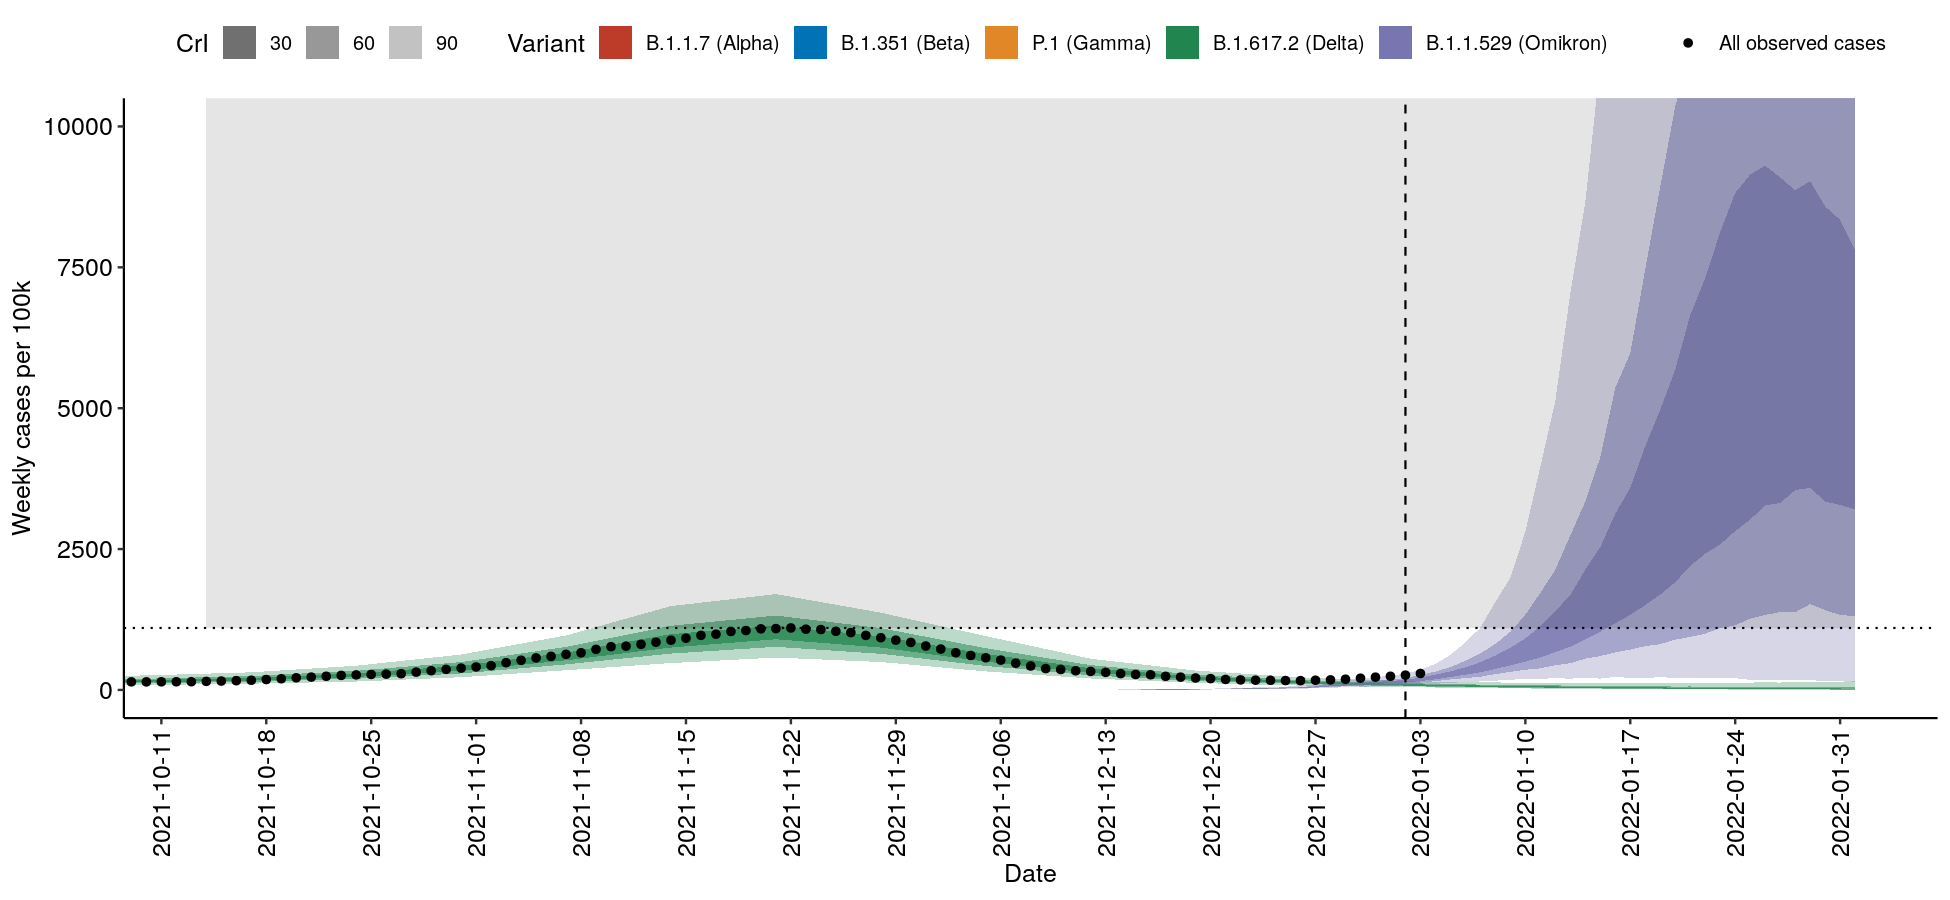
\includegraphics[width=1\linewidth]{omicron_austria_files/figure-latex/central-projection-1} \caption{Central scenario projection of cases for the Omicron and Delta variant. All observed cases shown as reported in the Austrian epidemiological surveillance system (EMS). Dashed line shows last day of data included in the fit. Grey area shows case numbers above previously observed case numbers, any actual observations in this region are likely to be affected by a reduction in ascertainment due to limited testing capacity.}\label{fig:central-projection}
\end{figure}

\begin{figure}
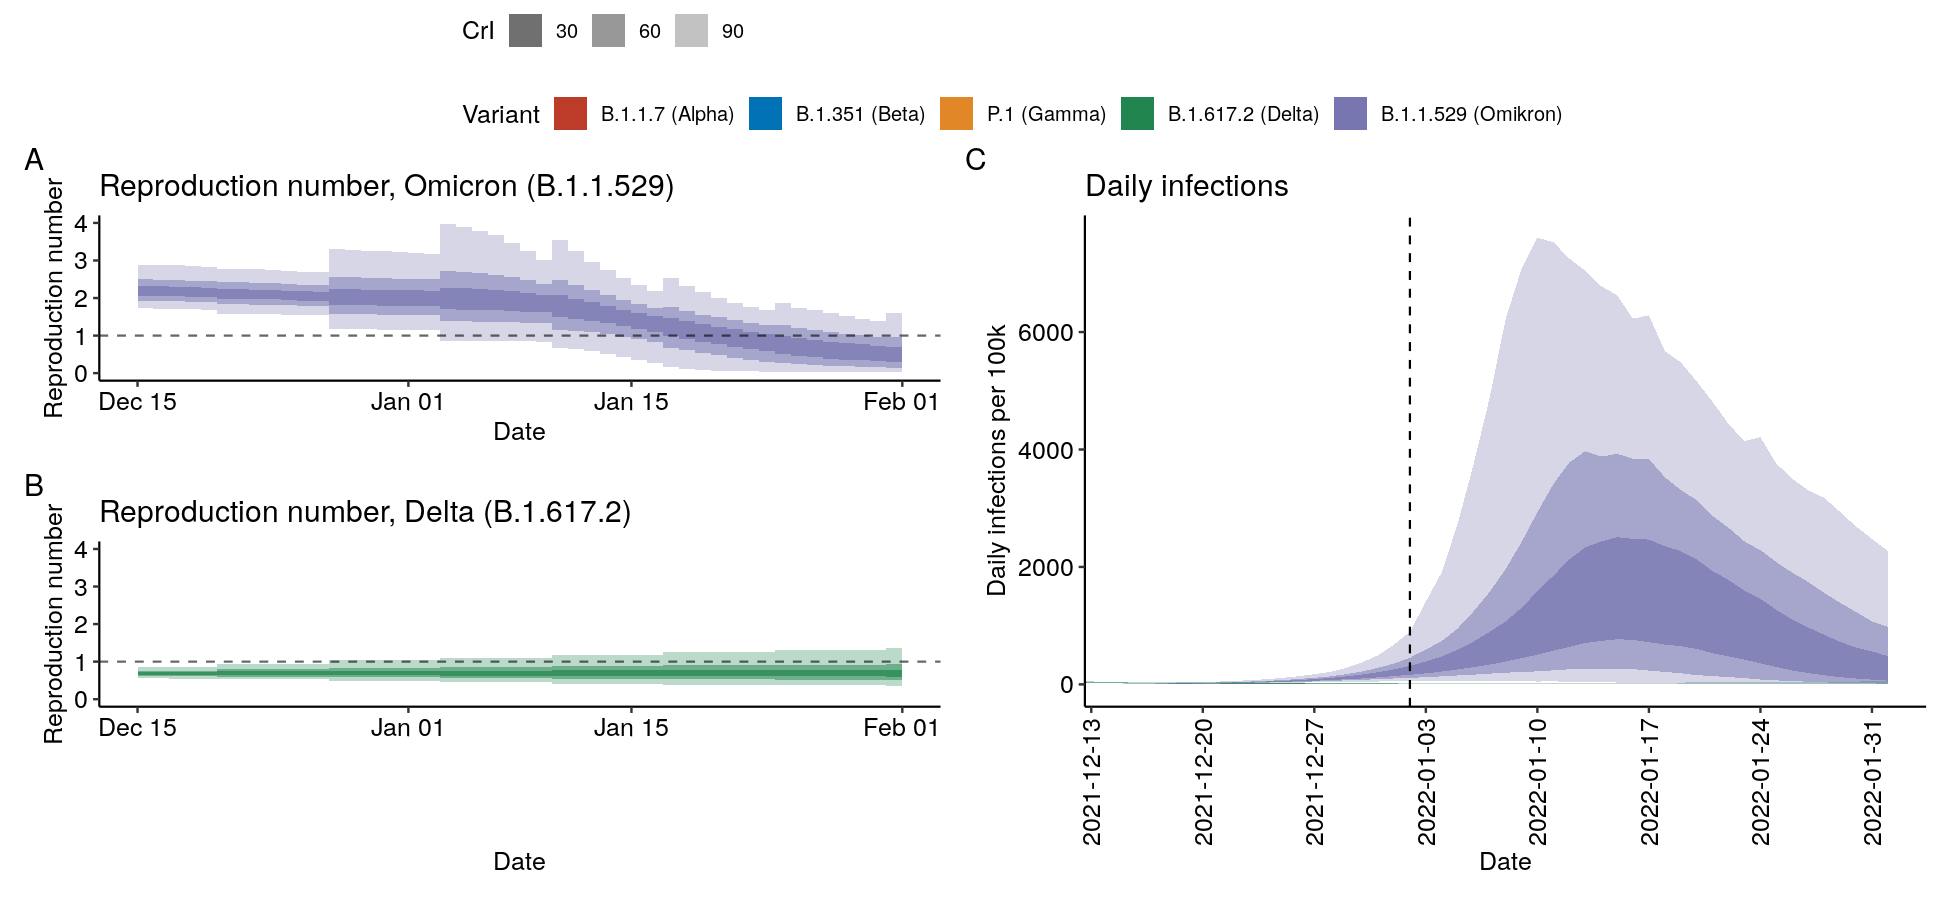
\includegraphics[width=1\linewidth]{omicron_austria_files/figure-latex/central-projection-rt-infections-1} \caption{A and B) Estimates of the time-varying reproduction number for (A) Omicron and (B) Delta. C) Projected daily infections per 100k population.}\label{fig:central-projection-rt-infections}
\end{figure}

\hypertarget{generation-time-scenarios}{%
\subsection{Generation time scenarios}\label{generation-time-scenarios}}

Since the generation time distribution is unclear, with some early evidence of a shorter serial interval. \autocite{SerialIntervalBasic}

The generation time distribution has been varied by assuming different mean, \(\mu\),
and standard deviation, \(\sigma\), variants for the discretized gamma distribution.
Where a mean of 4.6 days and standard deviation of 3.1 days match the assumptions for the Delta variant
and a mean of 3.13 days and standard deviation of 2.22 days is the central
assumption for the parameters of the generation time distribution of Omicron.

Both the incubation period and immunity in the population were fixed at the
central scenario assumptions.

\begin{figure}
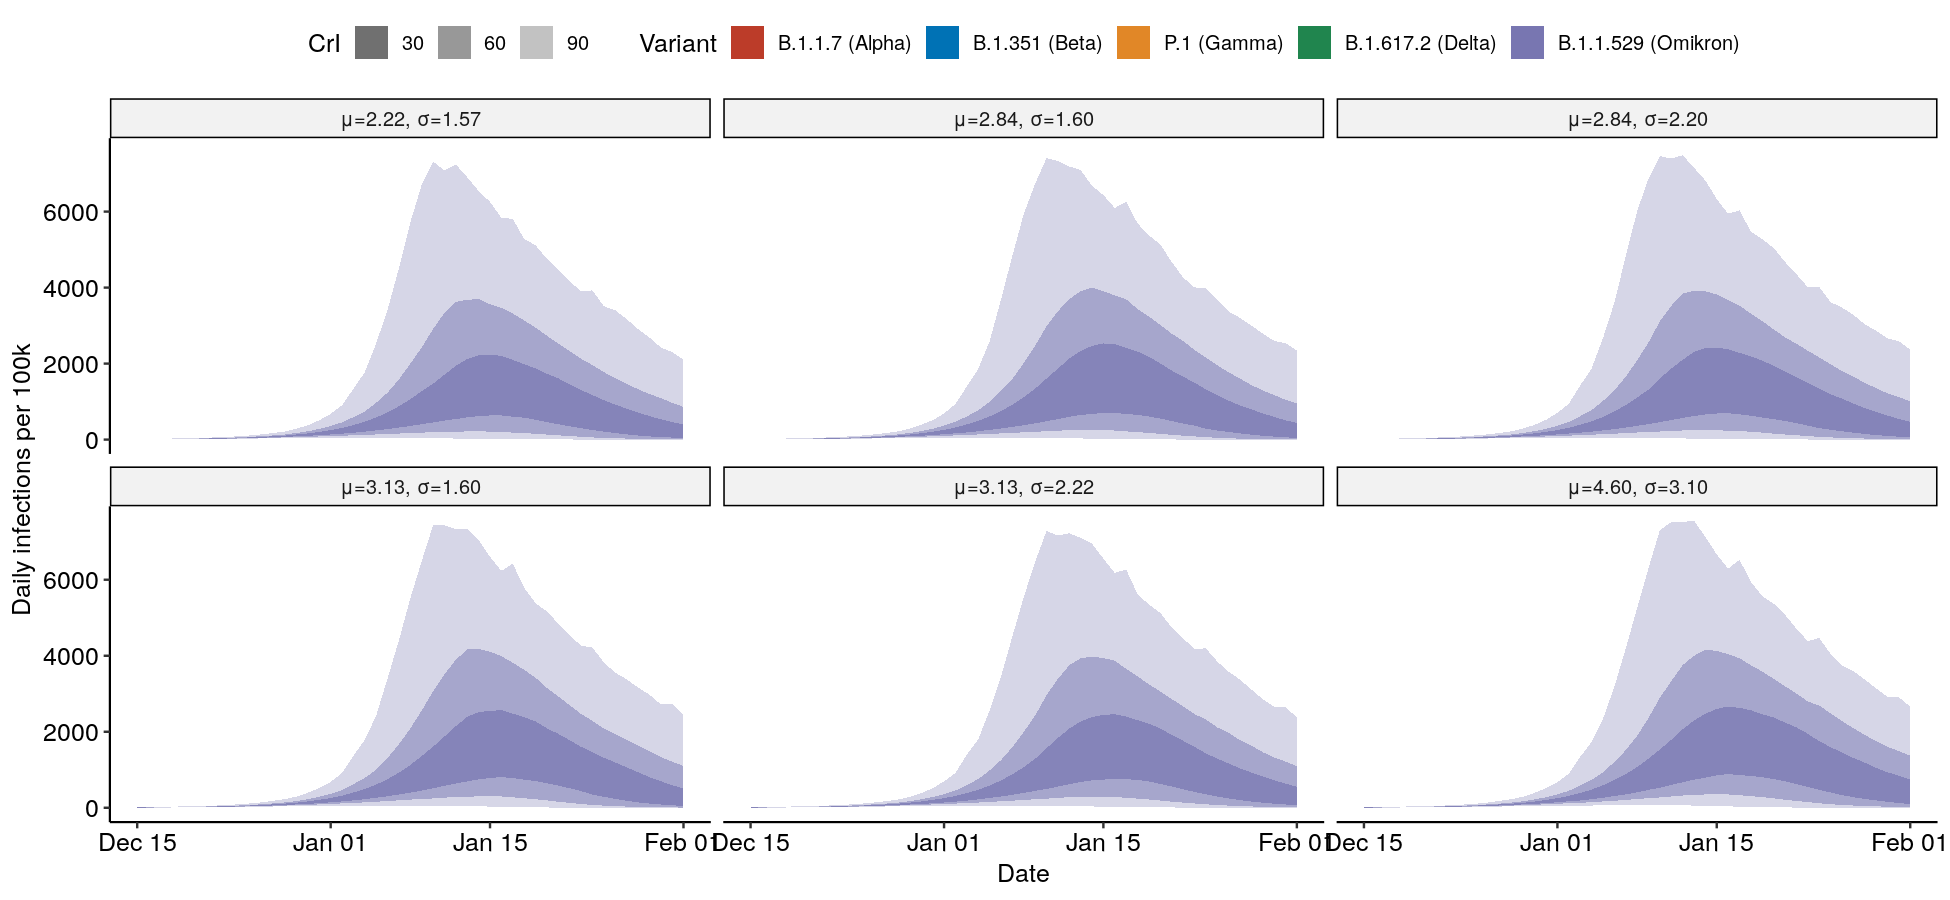
\includegraphics[width=1\linewidth]{omicron_austria_files/figure-latex/generation-time-scenarios-1} \caption{Projected daily infections for various assumptions of parameters of the generation distribution.}\label{fig:generation-time-scenarios}
\end{figure}

\hypertarget{multinomial-growth-advantage-of-omicron-over-delta}{%
\section{Multinomial growth advantage of Omicron over Delta}\label{multinomial-growth-advantage-of-omicron-over-delta}}

\hypertarget{methods-1}{%
\subsection{Methods}\label{methods-1}}

A Bayesian multinomial GLMM was specified using brms (version 2.16.3). Variant of concern data starting from the 1st of September 2021 for the following variants were included: Alpha (B.1.1.7), Delta (B.1.617.2) and Omicron (B.1.1.529) At the beginning of September 3 samples of Gamma (P.1) were also reported and 1 sample of Beta (B.1.351). Detection of other variants of concern has not been reported in Austria in the time period from 2021-09-01 to 2022-01-02. Estimates of CIs are Bayesian credible intervals estimated using highest density intervals.

A simple model structure with one growth rate and intercept per variant was used. An observation-level random effect was added to account for overdispersion\autocite{harrisonUsingObservationlevelRandom2014} in the VOC case data. Delta (B.1.617.2) was used as the reference variant for the model since it was detected over the whole time period.

\hypertarget{results-1}{%
\subsection{Results}\label{results-1}}

We estimate that Omicron (B.1.1.529) has a daily growth advantage of 0.23
(90\% ci 0.20 - 0.27) over Delta (B.1.617.2) in Austria.

\begin{figure}

{\centering 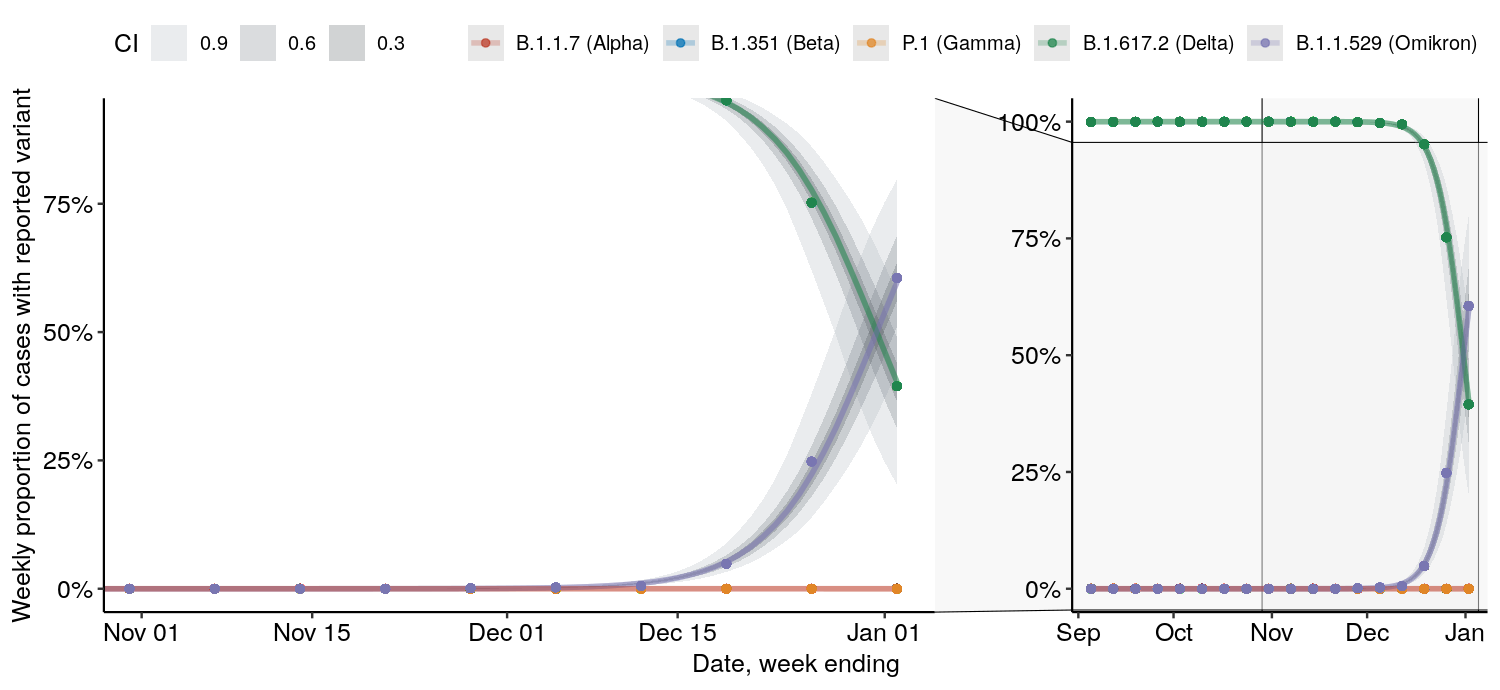
\includegraphics[width=0.8\linewidth]{omicron_austria_files/figure-latex/multinomial-fit-zoomed-1} 

}

\caption{Multinomial model fit.}\label{fig:multinomial-fit-zoomed}
\end{figure}

\begin{figure}

{\centering 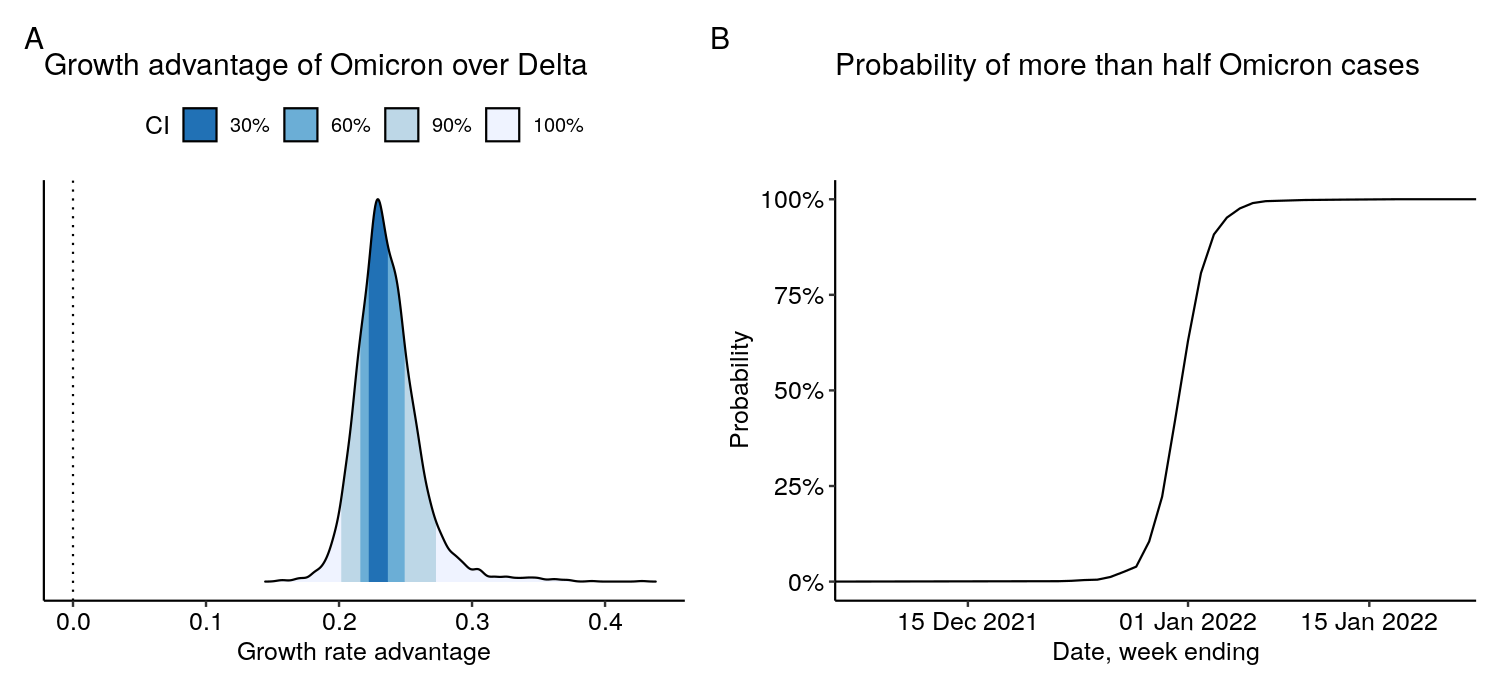
\includegraphics[width=0.8\linewidth]{omicron_austria_files/figure-latex/multinomial-growth-posterior-1} 

}

\caption{A: Estimated growth advantage of Omicron over Delta. B: Probability of Omicron making up half or more of the cases assigned to any variant.}\label{fig:multinomial-growth-posterior}
\end{figure}

\hypertarget{appendix-appendix}{%
\appendix}


\hypertarget{variant-sampling-in-austria}{%
\section{Variant sampling in Austria}\label{variant-sampling-in-austria}}

There have historically been large changes in the proportion of cases assigned to a VOC among all cases reported in Austria. Based upon sentinel full genome sequencing it can still be concluded that expect for the initial growth of Alpha over wild type infections one of the tracked VOCs was dominant in the respective time range.

\begin{figure}
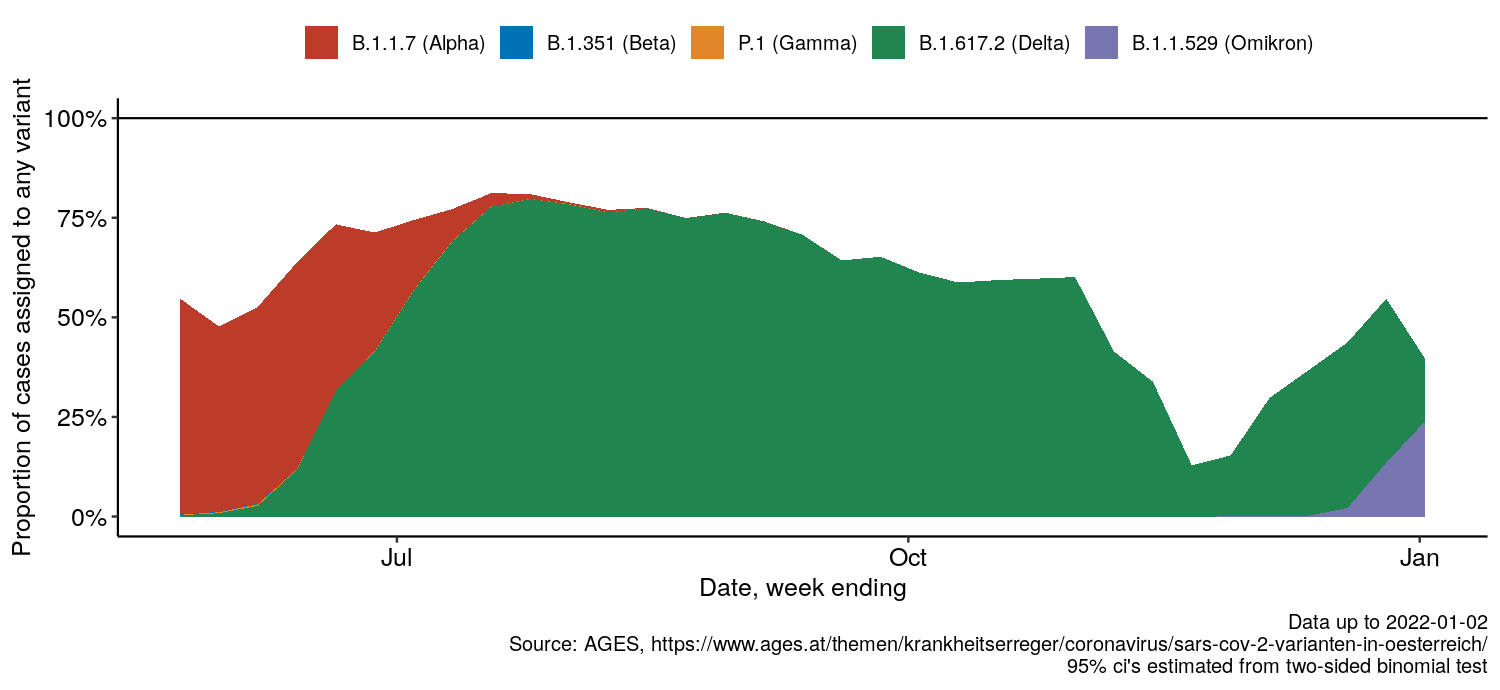
\includegraphics[width=1\linewidth]{omicron_austria_files/figure-latex/cases-assigned-voc-1} \caption{Proportion of cases assigned to each variant of all cases reported.}\label{fig:cases-assigned-voc}
\end{figure}

\hypertarget{full-model-fits-to-variant-cases}{%
\section{Full model fits to variant cases}\label{full-model-fits-to-variant-cases}}

Figures \ref{fig:epidemia-full-omicron-fit} and \ref{fig:epidemia-full-delta-fit} show the full model
fit for each variant.

\begin{figure}

{\centering 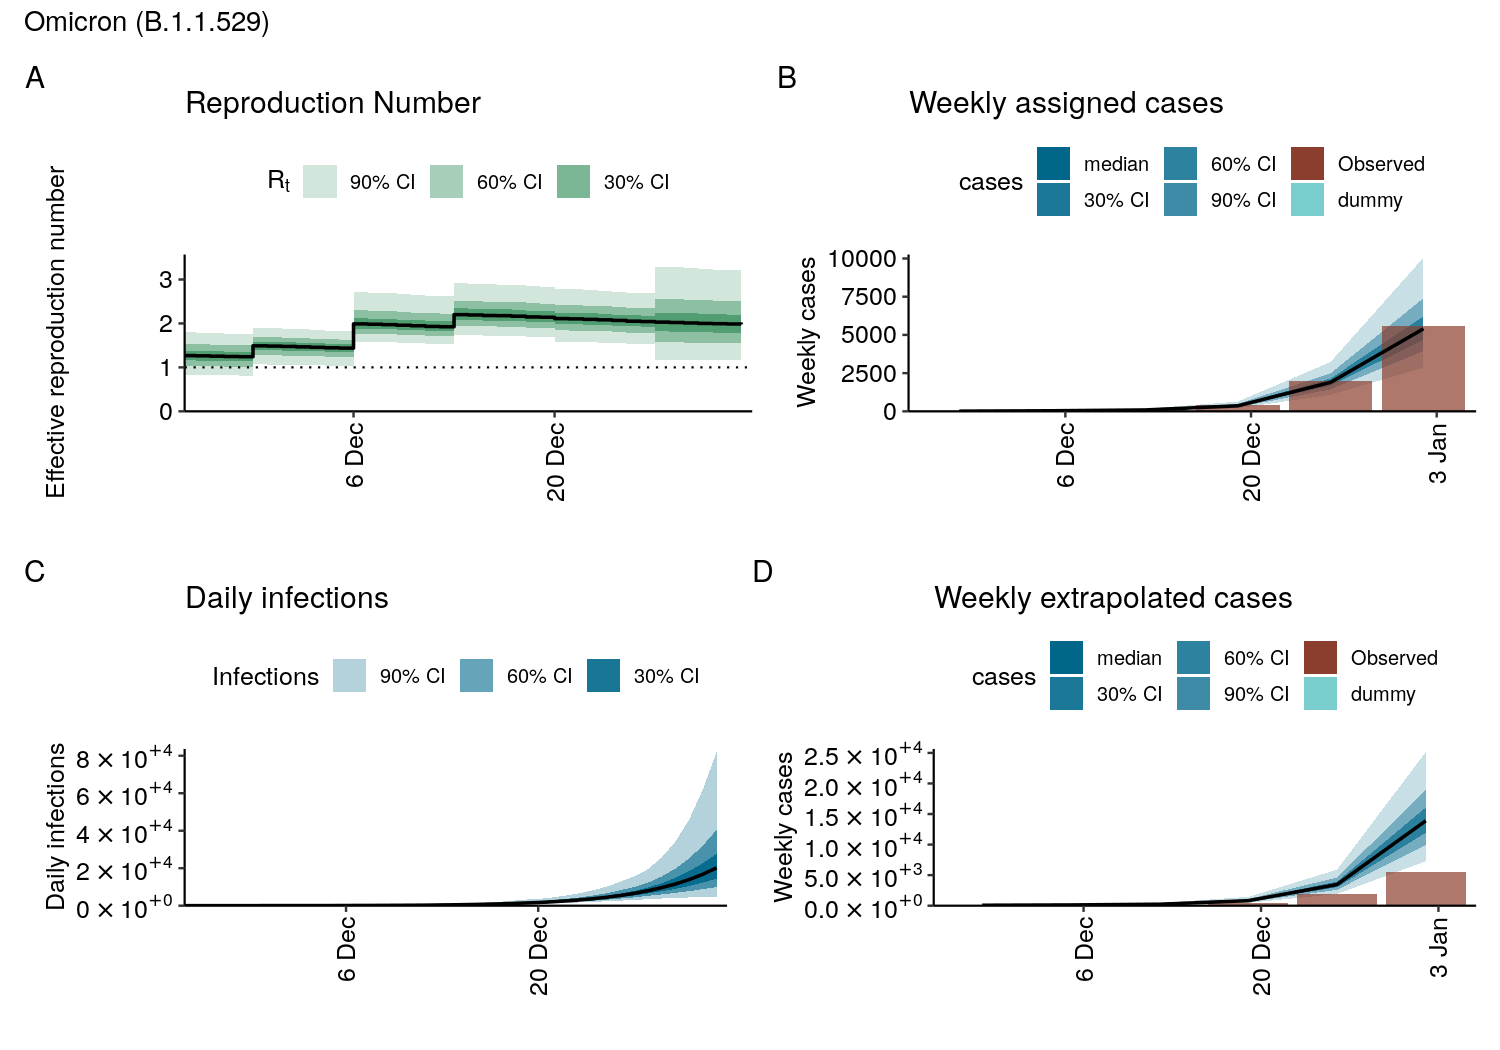
\includegraphics[width=0.8\linewidth]{omicron_austria_files/figure-latex/epidemia-full-omicron-fit-1} 

}

\caption{Full model fit}\label{fig:epidemia-full-omicron-fit}
\end{figure}

\begin{figure}

{\centering 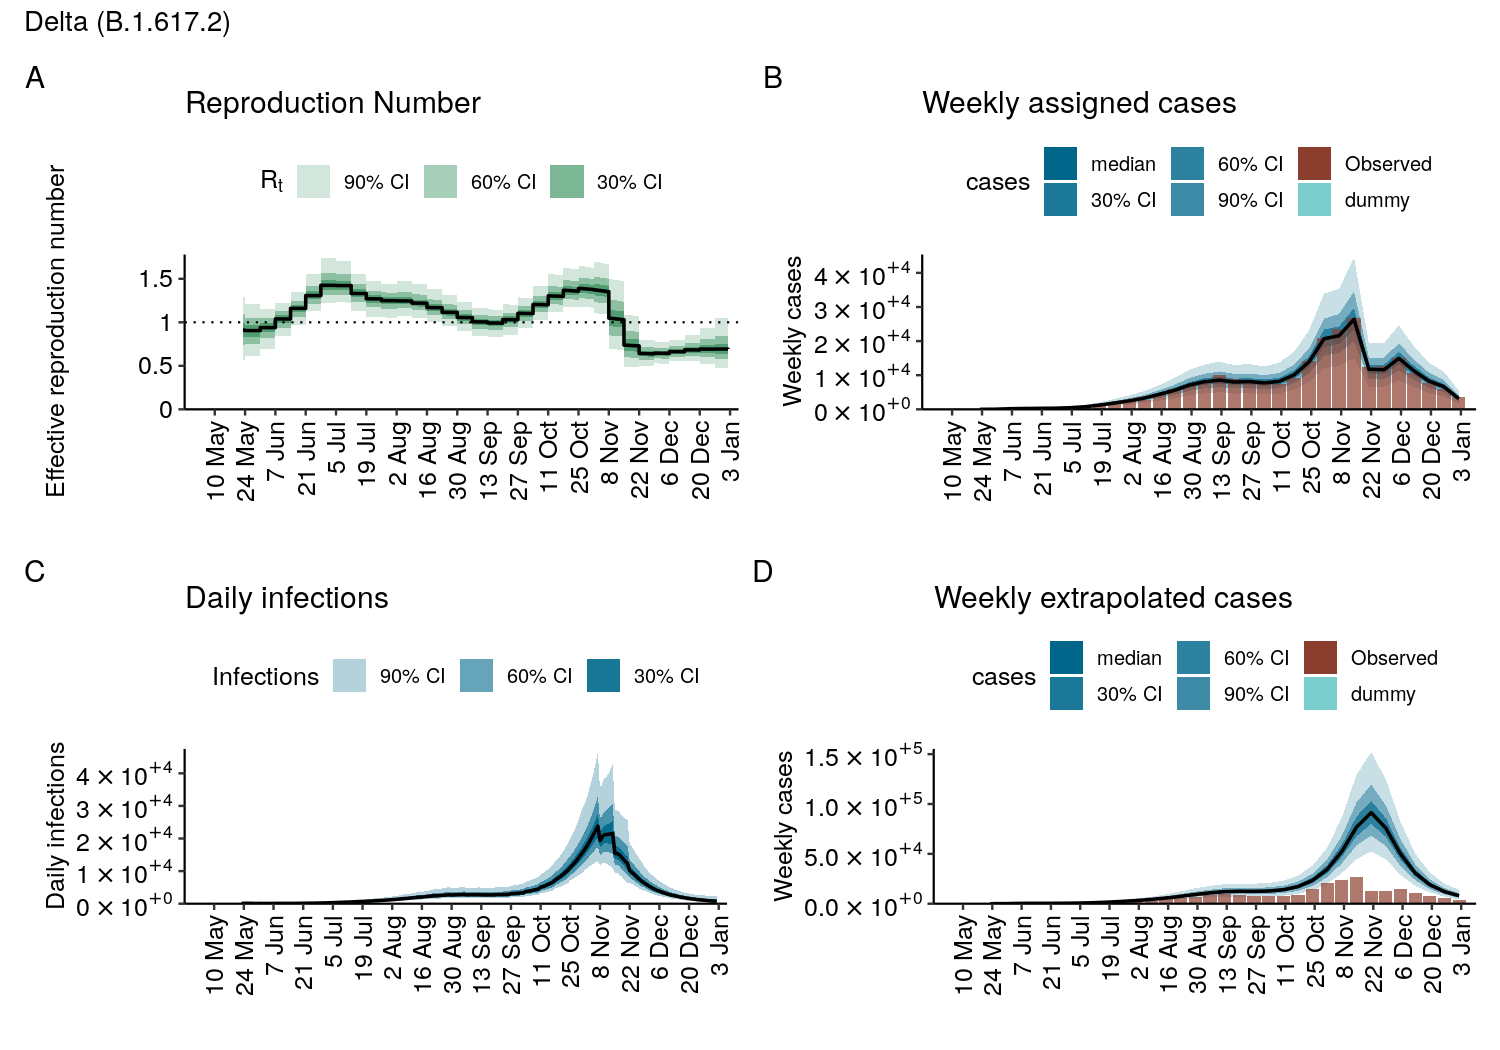
\includegraphics[width=0.8\linewidth]{omicron_austria_files/figure-latex/epidemia-full-delta-fit-1} 

}

\caption{Full model fit}\label{fig:epidemia-full-delta-fit}
\end{figure}

\hypertarget{immunity-and-vaccinations}{%
\section{Immunity and vaccinations}\label{immunity-and-vaccinations}}

\hypertarget{timeline-of-vaccinations-in-austria}{%
\subsection{Timeline of vaccinations in Austria}\label{timeline-of-vaccinations-in-austria}}

Figure \ref{fig:vaccine-doses-austria} shows the 7-day moving average of
daily doses of vaccines administered in Austria by manufacturer. \autocite{bmsgpkCOVID19ZeitreiheVerabreichten}

This data is used in the estimation of the immunity against infection
with the omicron variant.

\begin{figure}

{\centering 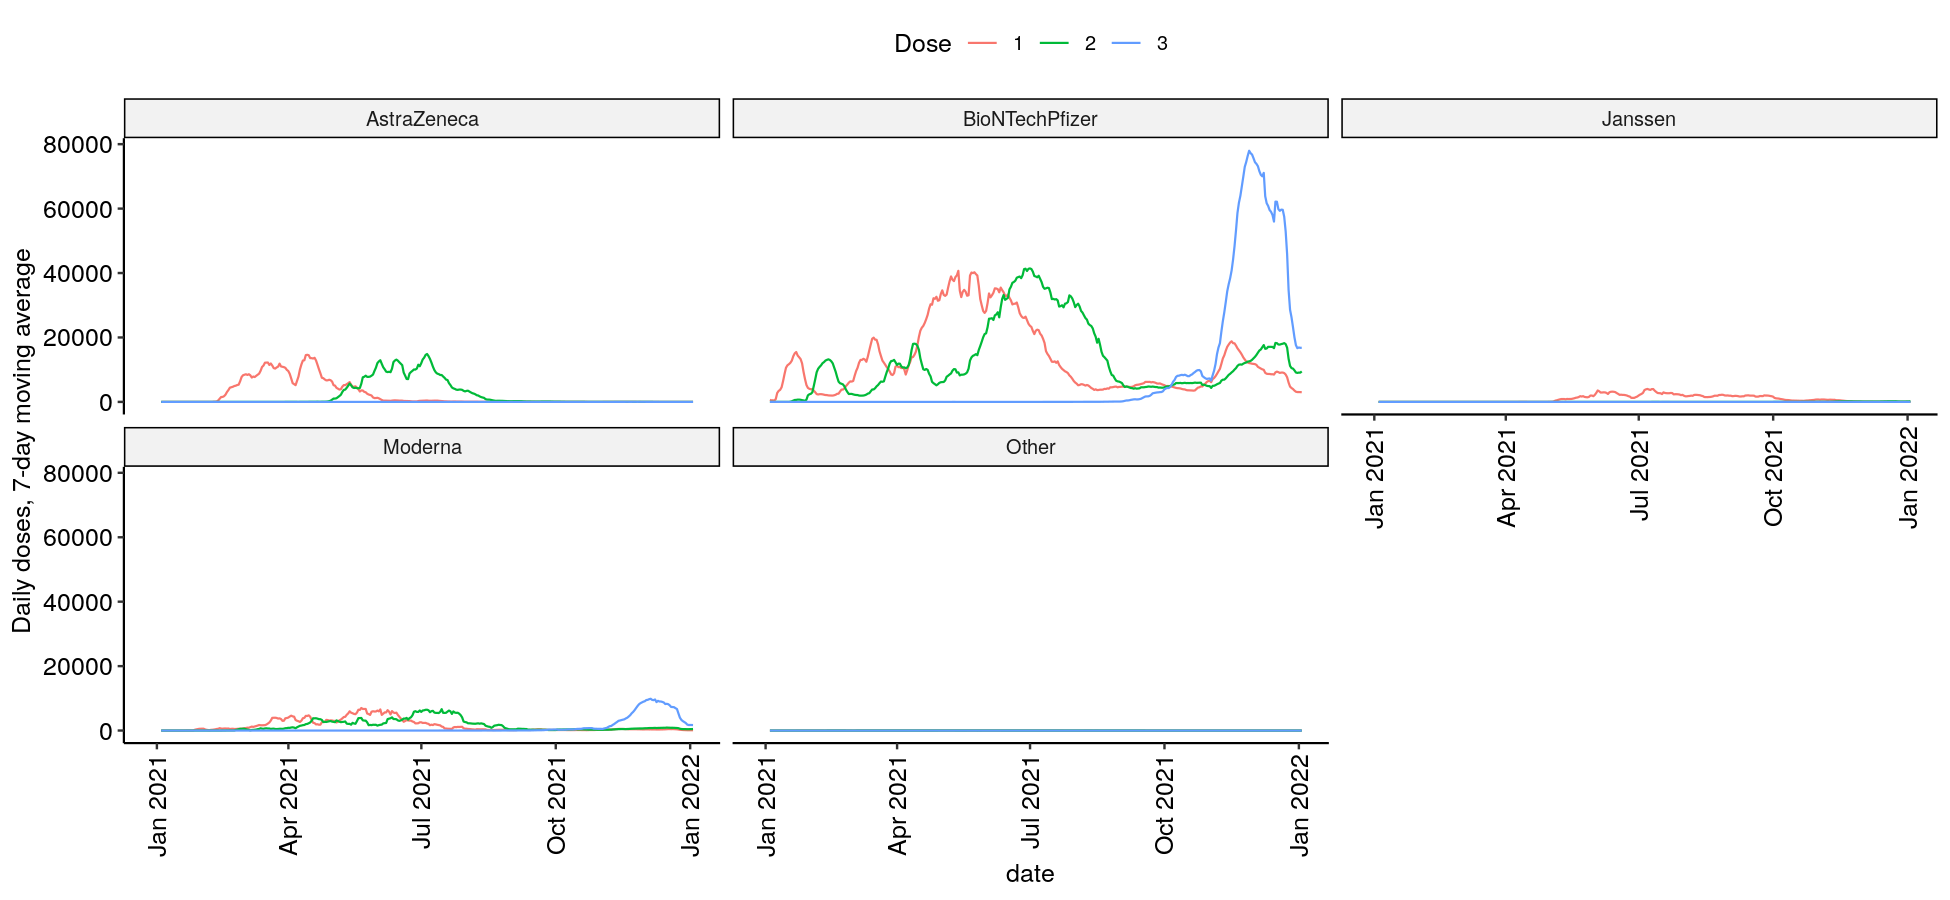
\includegraphics[width=1\linewidth]{omicron_austria_files/figure-latex/vaccine-doses-austria-1} 

}

\caption{Moving average (7-day) of vaccine doses administered in Austria, by manufacturer.}\label{fig:vaccine-doses-austria}
\end{figure}

\hypertarget{vaccine-effectiveness-against-infection-assumptions}{%
\subsection{Vaccine effectiveness against infection assumptions}\label{vaccine-effectiveness-against-infection-assumptions}}

A logit model based waning of vaccine effectivness
against infection with Omicron over time is assumed.

\begin{figure}

{\centering 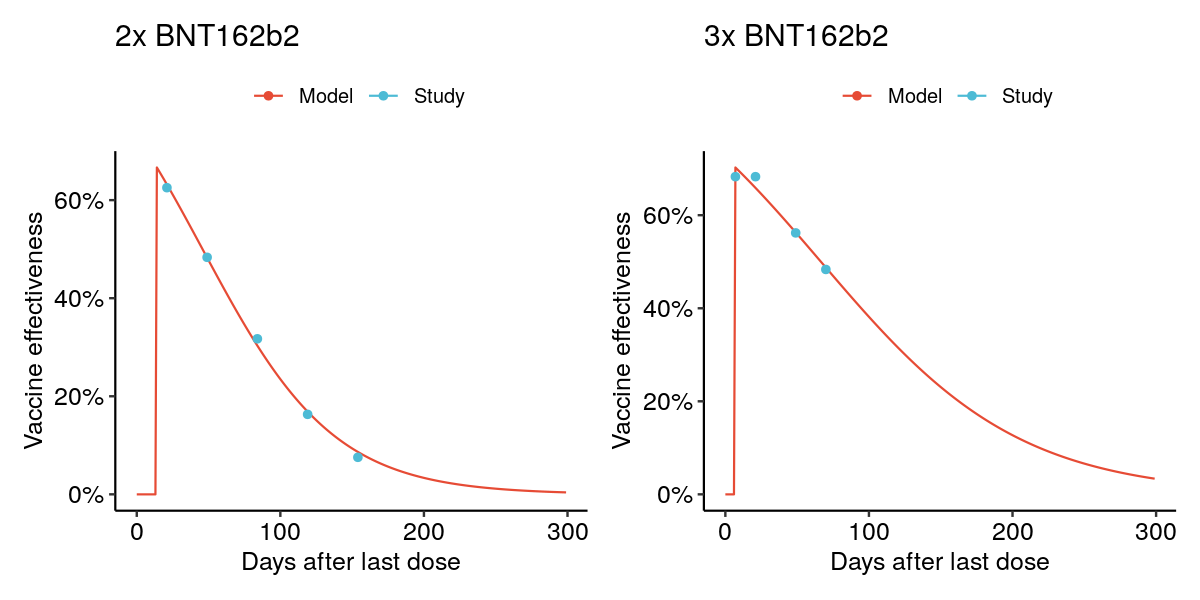
\includegraphics[width=0.75\linewidth]{omicron_austria_files/figure-latex/assumed-ve-1} 

}

\caption{Assumed vaccine effectivness against infection with the Omicron variant.}\label{fig:assumed-ve}
\end{figure}

\hypertarget{assumed-population-immunity-against-infection-with-omicron}{%
\subsection{Assumed population immunity against infection with Omicron}\label{assumed-population-immunity-against-infection-with-omicron}}

Figure \ref{fig:pop-immunity-omicron} shows the assumed immunity against infection with the Omicron variant
based upon the VE data.

\begin{figure}

{\centering 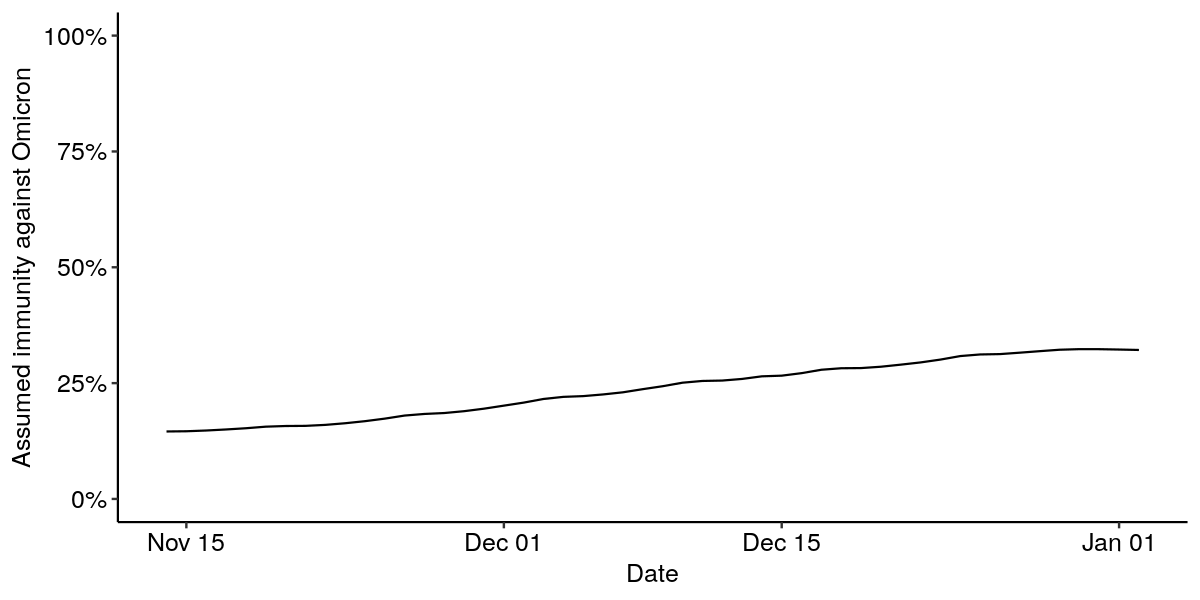
\includegraphics[width=0.75\linewidth]{omicron_austria_files/figure-latex/pop-immunity-omicron-1} 

}

\caption{Assumed immunity to the Omicron variant}\label{fig:pop-immunity-omicron}
\end{figure}

A large increase in immunity can be seen due to the Booster vaccination campaign
falling largely into the time period of Omicron introduction and establishment.

\hypertarget{time-distributions}{%
\section{Time distributions}\label{time-distributions}}

\hypertarget{infection-to-case-observation}{%
\subsection{Infection to case observation}\label{infection-to-case-observation}}

The assumed infection to case observation time distribution, obtained from combining the
incubation time distribution and case to lab diagnosis time distribution is shown in
figure \ref{fig:i2o-delta-omicron}.

The combined distribution was obtained by calculating the time delay from symptom onset
to case, by lab diagnosis date, taken from an anonymized line-listing. Random samples were
then drawn from an empirical distribution function of the time delay days obtained
from this dataset using the R package EnvStats. Those were combined with random
samples drawn from a gamma distribution assumed for the incubation period period
as described in section \ref{methods-incubation}.

\begin{figure}

{\centering 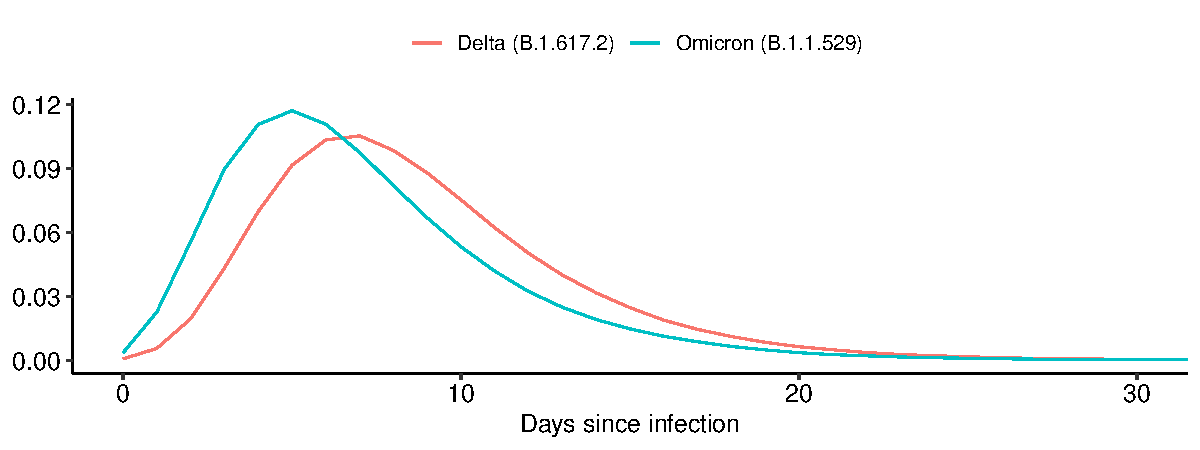
\includegraphics[width=0.75\linewidth]{omicron_austria_files/figure-latex/i2o-delta-omicron-1} 

}

\caption{Assumed infection to observation time distributions for Delta and Omicron}\label{fig:i2o-delta-omicron}
\end{figure}

\printbibliography[title=References]

\end{document}
